% Created by tikzDevice version 0.12.6 on 2026-05-15 10:04:31
% !TEX encoding = UTF-8 Unicode
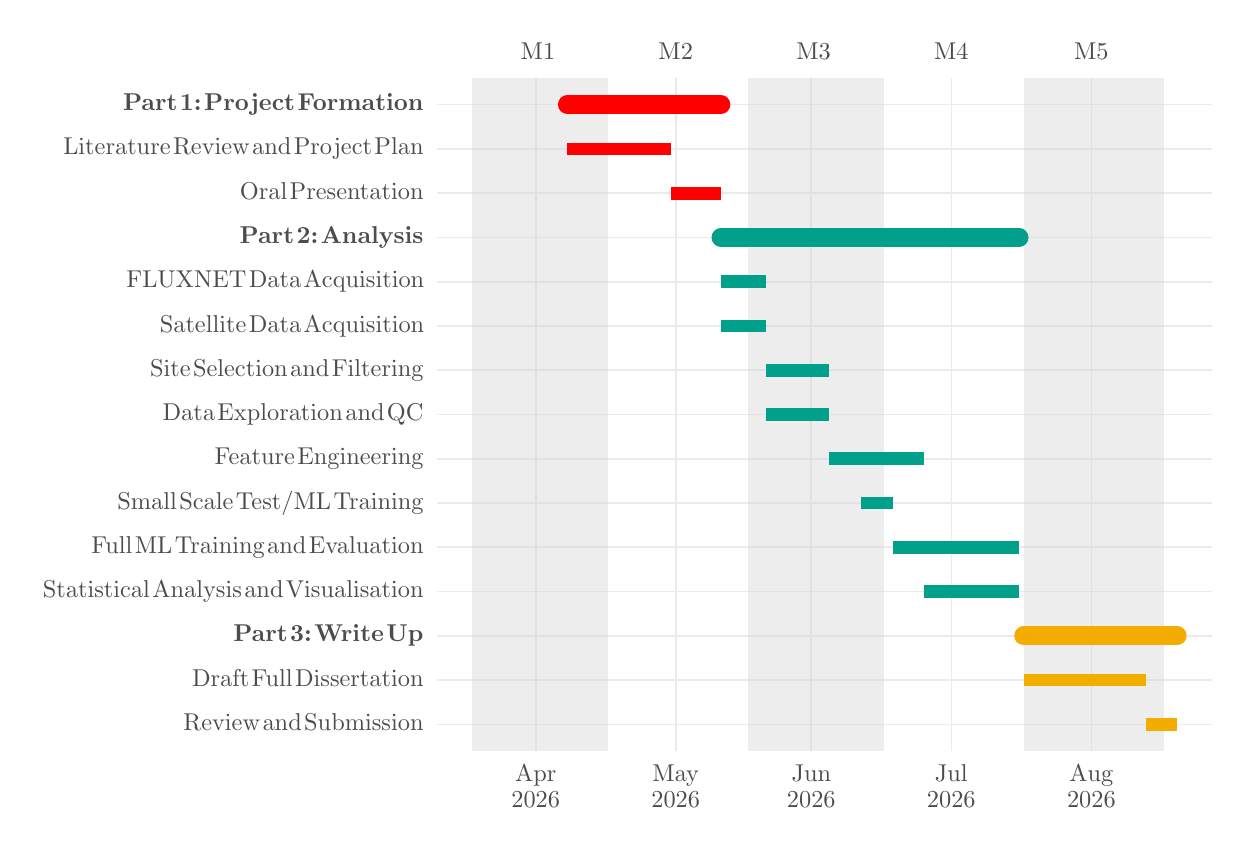
\begin{tikzpicture}[x=1pt,y=1pt]
\definecolor{fillColor}{RGB}{255,255,255}
\path[use as bounding box,fill=fillColor,fill opacity=0.00] (0,0) rectangle (433.62,289.08);
\begin{scope}
\path[clip] (  0.00,  0.00) rectangle (433.62,289.08);
\definecolor{fillColor}{RGB}{255,255,255}

\path[fill=fillColor] (  0.00,  0.00) rectangle (433.62,289.08);
\end{scope}
\begin{scope}
\path[clip] (147.99, 27.73) rectangle (428.12,270.86);
\definecolor{drawColor}{gray}{0.92}

\path[draw=drawColor,line width= 0.6pt,line join=round] (147.99, 37.32) --
	(428.12, 37.32);

\path[draw=drawColor,line width= 0.6pt,line join=round] (147.99, 53.32) --
	(428.12, 53.32);

\path[draw=drawColor,line width= 0.6pt,line join=round] (147.99, 69.31) --
	(428.12, 69.31);

\path[draw=drawColor,line width= 0.6pt,line join=round] (147.99, 85.31) --
	(428.12, 85.31);

\path[draw=drawColor,line width= 0.6pt,line join=round] (147.99,101.31) --
	(428.12,101.31);

\path[draw=drawColor,line width= 0.6pt,line join=round] (147.99,117.30) --
	(428.12,117.30);

\path[draw=drawColor,line width= 0.6pt,line join=round] (147.99,133.30) --
	(428.12,133.30);

\path[draw=drawColor,line width= 0.6pt,line join=round] (147.99,149.29) --
	(428.12,149.29);

\path[draw=drawColor,line width= 0.6pt,line join=round] (147.99,165.29) --
	(428.12,165.29);

\path[draw=drawColor,line width= 0.6pt,line join=round] (147.99,181.28) --
	(428.12,181.28);

\path[draw=drawColor,line width= 0.6pt,line join=round] (147.99,197.28) --
	(428.12,197.28);

\path[draw=drawColor,line width= 0.6pt,line join=round] (147.99,213.27) --
	(428.12,213.27);

\path[draw=drawColor,line width= 0.6pt,line join=round] (147.99,229.27) --
	(428.12,229.27);

\path[draw=drawColor,line width= 0.6pt,line join=round] (147.99,245.27) --
	(428.12,245.27);

\path[draw=drawColor,line width= 0.6pt,line join=round] (147.99,261.26) --
	(428.12,261.26);

\path[draw=drawColor,line width= 0.6pt,line join=round] (183.58, 27.73) --
	(183.58,270.86);

\path[draw=drawColor,line width= 0.6pt,line join=round] (234.18, 27.73) --
	(234.18,270.86);

\path[draw=drawColor,line width= 0.6pt,line join=round] (283.16, 27.73) --
	(283.16,270.86);

\path[draw=drawColor,line width= 0.6pt,line join=round] (333.76, 27.73) --
	(333.76,270.86);

\path[draw=drawColor,line width= 0.6pt,line join=round] (384.37, 27.73) --
	(384.37,270.86);
\definecolor{fillColor}{RGB}{211,211,211}

\path[fill=fillColor,fill opacity=0.40] (160.72, 27.73) rectangle (209.70,270.86);

\path[fill=fillColor,fill opacity=0.40] (260.30, 27.73) rectangle (309.28,270.86);

\path[fill=fillColor,fill opacity=0.40] (359.88, 27.73) rectangle (410.49,270.86);
\definecolor{drawColor}{RGB}{242,173,0}

\path[draw=drawColor,line width= 4.6pt,line join=round] (403.96, 37.32) -- (415.39, 37.32);

\path[draw=drawColor,line width= 4.6pt,line join=round] (359.88, 53.32) -- (403.96, 53.32);

\path[] (359.88, 69.31) -- (415.39, 69.31);
\definecolor{drawColor}{RGB}{0,160,138}

\path[draw=drawColor,line width= 4.6pt,line join=round] (323.97, 85.31) -- (358.25, 85.31);

\path[draw=drawColor,line width= 4.6pt,line join=round] (312.54,101.31) -- (358.25,101.31);

\path[draw=drawColor,line width= 4.6pt,line join=round] (301.12,117.30) -- (312.54,117.30);

\path[draw=drawColor,line width= 4.6pt,line join=round] (289.69,133.30) -- (323.97,133.30);

\path[draw=drawColor,line width= 4.6pt,line join=round] (266.83,149.29) -- (289.69,149.29);

\path[draw=drawColor,line width= 4.6pt,line join=round] (266.83,165.29) -- (289.69,165.29);

\path[draw=drawColor,line width= 4.6pt,line join=round] (250.51,181.28) -- (266.83,181.28);

\path[draw=drawColor,line width= 4.6pt,line join=round] (250.51,197.28) -- (266.83,197.28);

\path[] (250.51,213.27) -- (358.25,213.27);
\definecolor{drawColor}{RGB}{255,0,0}

\path[draw=drawColor,line width= 4.6pt,line join=round] (232.55,229.27) -- (250.51,229.27);

\path[draw=drawColor,line width= 4.6pt,line join=round] (195.01,245.27) -- (232.55,245.27);

\path[] (195.01,261.26) -- (250.51,261.26);

\path[] (403.96, 37.32) -- (415.39, 37.32);

\path[] (359.88, 53.32) -- (403.96, 53.32);
\definecolor{drawColor}{RGB}{242,173,0}

\path[draw=drawColor,line width= 6.8pt,line join=round,line cap=round] (359.88, 69.31) -- (415.39, 69.31);

\path[] (323.97, 85.31) -- (358.25, 85.31);

\path[] (312.54,101.31) -- (358.25,101.31);

\path[] (301.12,117.30) -- (312.54,117.30);

\path[] (289.69,133.30) -- (323.97,133.30);

\path[] (266.83,149.29) -- (289.69,149.29);

\path[] (266.83,165.29) -- (289.69,165.29);

\path[] (250.51,181.28) -- (266.83,181.28);

\path[] (250.51,197.28) -- (266.83,197.28);
\definecolor{drawColor}{RGB}{0,160,138}

\path[draw=drawColor,line width= 6.8pt,line join=round,line cap=round] (250.51,213.27) -- (358.25,213.27);

\path[] (232.55,229.27) -- (250.51,229.27);

\path[] (195.01,245.27) -- (232.55,245.27);
\definecolor{drawColor}{RGB}{255,0,0}

\path[draw=drawColor,line width= 6.8pt,line join=round,line cap=round] (195.01,261.26) -- (250.51,261.26);
\end{scope}
\begin{scope}
\path[clip] (  0.00,  0.00) rectangle (433.62,289.08);
\definecolor{drawColor}{gray}{0.30}

\node[text=drawColor,anchor=base,inner sep=0pt, outer sep=0pt, scale=  0.88] at (184.39,277.52) {M1};

\node[text=drawColor,anchor=base,inner sep=0pt, outer sep=0pt, scale=  0.88] at (234.18,277.52) {M2};

\node[text=drawColor,anchor=base,inner sep=0pt, outer sep=0pt, scale=  0.88] at (283.97,277.52) {M3};

\node[text=drawColor,anchor=base,inner sep=0pt, outer sep=0pt, scale=  0.88] at (333.76,277.52) {M4};

\node[text=drawColor,anchor=base,inner sep=0pt, outer sep=0pt, scale=  0.88] at (384.37,277.52) {M5};
\end{scope}
\begin{scope}
\path[clip] (  0.00,  0.00) rectangle (433.62,289.08);
\definecolor{drawColor}{gray}{0.30}

\node[text=drawColor,anchor=base west,inner sep=0pt, outer sep=0pt, scale=  0.88] at ( 56.26, 35.15) {Review};

\node[text=drawColor,anchor=base west,inner sep=0pt, outer sep=0pt, scale=  0.88] at ( 84.88, 35.15) {and};

\node[text=drawColor,anchor=base west,inner sep=0pt, outer sep=0pt, scale=  0.88] at ( 99.93, 35.15) {Submission};
\end{scope}
\begin{scope}
\path[clip] (  0.00,  0.00) rectangle (433.62,289.08);
\definecolor{drawColor}{gray}{0.30}

\node[text=drawColor,anchor=base west,inner sep=0pt, outer sep=0pt, scale=  0.88] at ( 59.39, 51.14) {Draft};

\node[text=drawColor,anchor=base west,inner sep=0pt, outer sep=0pt, scale=  0.88] at ( 80.94, 51.14) {Full};

\node[text=drawColor,anchor=base west,inner sep=0pt, outer sep=0pt, scale=  0.88] at ( 96.61, 51.14) {Dissertation};
\end{scope}
\begin{scope}
\path[clip] (  0.00,  0.00) rectangle (433.62,289.08);
\definecolor{drawColor}{gray}{0.30}

\node[text=drawColor,anchor=base west,inner sep=0pt, outer sep=0pt, scale=  0.88] at ( 74.31, 67.13) {\bfseries Part};

\node[text=drawColor,anchor=base west,inner sep=0pt, outer sep=0pt, scale=  0.88] at ( 94.84, 67.13) {\bfseries 3:};

\node[text=drawColor,anchor=base west,inner sep=0pt, outer sep=0pt, scale=  0.88] at (103.59, 67.13) {\bfseries Write};

\node[text=drawColor,anchor=base west,inner sep=0pt, outer sep=0pt, scale=  0.88] at (129.64, 67.13) {\bfseries Up};
\end{scope}
\begin{scope}
\path[clip] (  0.00,  0.00) rectangle (433.62,289.08);
\definecolor{drawColor}{gray}{0.30}

\node[text=drawColor,anchor=base west,inner sep=0pt, outer sep=0pt, scale=  0.88] at (  5.50, 83.13) {Statistical};

\node[text=drawColor,anchor=base west,inner sep=0pt, outer sep=0pt, scale=  0.88] at ( 45.04, 83.13) {Analysis};

\node[text=drawColor,anchor=base west,inner sep=0pt, outer sep=0pt, scale=  0.88] at ( 78.28, 83.13) {and};

\node[text=drawColor,anchor=base west,inner sep=0pt, outer sep=0pt, scale=  0.88] at ( 93.33, 83.13) {Visualisation};
\end{scope}
\begin{scope}
\path[clip] (  0.00,  0.00) rectangle (433.62,289.08);
\definecolor{drawColor}{gray}{0.30}

\node[text=drawColor,anchor=base west,inner sep=0pt, outer sep=0pt, scale=  0.88] at ( 23.05, 99.13) {Full};

\node[text=drawColor,anchor=base west,inner sep=0pt, outer sep=0pt, scale=  0.88] at ( 38.71, 99.13) {ML};

\node[text=drawColor,anchor=base west,inner sep=0pt, outer sep=0pt, scale=  0.88] at ( 53.16, 99.13) {Training};

\node[text=drawColor,anchor=base west,inner sep=0pt, outer sep=0pt, scale=  0.88] at ( 86.56, 99.13) {and};

\node[text=drawColor,anchor=base west,inner sep=0pt, outer sep=0pt, scale=  0.88] at (101.62, 99.13) {Evaluation};
\end{scope}
\begin{scope}
\path[clip] (  0.00,  0.00) rectangle (433.62,289.08);
\definecolor{drawColor}{gray}{0.30}

\node[text=drawColor,anchor=base west,inner sep=0pt, outer sep=0pt, scale=  0.88] at ( 32.43,115.13) {Small};

\node[text=drawColor,anchor=base west,inner sep=0pt, outer sep=0pt, scale=  0.88] at ( 54.82,115.13) {Scale};

\node[text=drawColor,anchor=base west,inner sep=0pt, outer sep=0pt, scale=  0.88] at ( 75.25,115.13) {Test/ML};

\node[text=drawColor,anchor=base west,inner sep=0pt, outer sep=0pt, scale=  0.88] at (110.51,115.13) {Training};
\end{scope}
\begin{scope}
\path[clip] (  0.00,  0.00) rectangle (433.62,289.08);
\definecolor{drawColor}{gray}{0.30}

\node[text=drawColor,anchor=base west,inner sep=0pt, outer sep=0pt, scale=  0.88] at ( 67.57,131.12) {Feature};

\node[text=drawColor,anchor=base west,inner sep=0pt, outer sep=0pt, scale=  0.88] at ( 97.44,131.12) {Engineering};
\end{scope}
\begin{scope}
\path[clip] (  0.00,  0.00) rectangle (433.62,289.08);
\definecolor{drawColor}{gray}{0.30}

\node[text=drawColor,anchor=base west,inner sep=0pt, outer sep=0pt, scale=  0.88] at ( 48.73,147.12) {Data};

\node[text=drawColor,anchor=base west,inner sep=0pt, outer sep=0pt, scale=  0.88] at ( 68.55,147.12) {Exploration};

\node[text=drawColor,anchor=base west,inner sep=0pt, outer sep=0pt, scale=  0.88] at (114.79,147.12) {and};

\node[text=drawColor,anchor=base west,inner sep=0pt, outer sep=0pt, scale=  0.88] at (129.84,147.12) {QC};
\end{scope}
\begin{scope}
\path[clip] (  0.00,  0.00) rectangle (433.62,289.08);
\definecolor{drawColor}{gray}{0.30}

\node[text=drawColor,anchor=base west,inner sep=0pt, outer sep=0pt, scale=  0.88] at ( 44.21,163.11) {Site};

\node[text=drawColor,anchor=base west,inner sep=0pt, outer sep=0pt, scale=  0.88] at ( 59.75,163.11) {Selection};

\node[text=drawColor,anchor=base west,inner sep=0pt, outer sep=0pt, scale=  0.88] at ( 94.85,163.11) {and};

\node[text=drawColor,anchor=base west,inner sep=0pt, outer sep=0pt, scale=  0.88] at (109.90,163.11) {Filtering};
\end{scope}
\begin{scope}
\path[clip] (  0.00,  0.00) rectangle (433.62,289.08);
\definecolor{drawColor}{gray}{0.30}

\node[text=drawColor,anchor=base west,inner sep=0pt, outer sep=0pt, scale=  0.88] at ( 47.75,179.11) {Satellite};

\node[text=drawColor,anchor=base west,inner sep=0pt, outer sep=0pt, scale=  0.88] at ( 79.92,179.11) {Data};

\node[text=drawColor,anchor=base west,inner sep=0pt, outer sep=0pt, scale=  0.88] at ( 99.74,179.11) {Acquisition};
\end{scope}
\begin{scope}
\path[clip] (  0.00,  0.00) rectangle (433.62,289.08);
\definecolor{drawColor}{gray}{0.30}

\node[text=drawColor,anchor=base west,inner sep=0pt, outer sep=0pt, scale=  0.88] at ( 35.66,195.10) {FLUXNET};

\node[text=drawColor,anchor=base west,inner sep=0pt, outer sep=0pt, scale=  0.88] at ( 79.92,195.10) {Data};

\node[text=drawColor,anchor=base west,inner sep=0pt, outer sep=0pt, scale=  0.88] at ( 99.74,195.10) {Acquisition};
\end{scope}
\begin{scope}
\path[clip] (  0.00,  0.00) rectangle (433.62,289.08);
\definecolor{drawColor}{gray}{0.30}

\node[text=drawColor,anchor=base west,inner sep=0pt, outer sep=0pt, scale=  0.88] at ( 76.63,211.09) {\bfseries Part};

\node[text=drawColor,anchor=base west,inner sep=0pt, outer sep=0pt, scale=  0.88] at ( 97.16,211.09) {\bfseries 2:};

\node[text=drawColor,anchor=base west,inner sep=0pt, outer sep=0pt, scale=  0.88] at (105.91,211.09) {\bfseries Analysis};
\end{scope}
\begin{scope}
\path[clip] (  0.00,  0.00) rectangle (433.62,289.08);
\definecolor{drawColor}{gray}{0.30}

\node[text=drawColor,anchor=base west,inner sep=0pt, outer sep=0pt, scale=  0.88] at ( 76.69,227.09) {Oral};

\node[text=drawColor,anchor=base west,inner sep=0pt, outer sep=0pt, scale=  0.88] at ( 94.70,227.09) {Presentation};
\end{scope}
\begin{scope}
\path[clip] (  0.00,  0.00) rectangle (433.62,289.08);
\definecolor{drawColor}{gray}{0.30}

\node[text=drawColor,anchor=base west,inner sep=0pt, outer sep=0pt, scale=  0.88] at ( 12.86,243.09) {Literature};

\node[text=drawColor,anchor=base west,inner sep=0pt, outer sep=0pt, scale=  0.88] at ( 52.52,243.09) {Review};

\node[text=drawColor,anchor=base west,inner sep=0pt, outer sep=0pt, scale=  0.88] at ( 81.14,243.09) {and};

\node[text=drawColor,anchor=base west,inner sep=0pt, outer sep=0pt, scale=  0.88] at ( 96.19,243.09) {Project};

\node[text=drawColor,anchor=base west,inner sep=0pt, outer sep=0pt, scale=  0.88] at (125.32,243.09) {Plan};
\end{scope}
\begin{scope}
\path[clip] (  0.00,  0.00) rectangle (433.62,289.08);
\definecolor{drawColor}{gray}{0.30}

\node[text=drawColor,anchor=base west,inner sep=0pt, outer sep=0pt, scale=  0.88] at ( 34.49,259.08) {\bfseries Part};

\node[text=drawColor,anchor=base west,inner sep=0pt, outer sep=0pt, scale=  0.88] at ( 55.03,259.08) {\bfseries 1:};

\node[text=drawColor,anchor=base west,inner sep=0pt, outer sep=0pt, scale=  0.88] at ( 63.77,259.08) {\bfseries Project};

\node[text=drawColor,anchor=base west,inner sep=0pt, outer sep=0pt, scale=  0.88] at ( 97.52,259.08) {\bfseries Formation};
\end{scope}
\begin{scope}
\path[clip] (  0.00,  0.00) rectangle (433.62,289.08);
\definecolor{drawColor}{gray}{0.30}

\node[text=drawColor,anchor=base,inner sep=0pt, outer sep=0pt, scale=  0.88] at (183.58, 16.71) {Apr};

\node[text=drawColor,anchor=base,inner sep=0pt, outer sep=0pt, scale=  0.88] at (183.58,  7.21) {2026};

\node[text=drawColor,anchor=base,inner sep=0pt, outer sep=0pt, scale=  0.88] at (234.18, 16.71) {May};

\node[text=drawColor,anchor=base,inner sep=0pt, outer sep=0pt, scale=  0.88] at (234.18,  7.21) {2026};

\node[text=drawColor,anchor=base,inner sep=0pt, outer sep=0pt, scale=  0.88] at (283.16, 16.71) {Jun};

\node[text=drawColor,anchor=base,inner sep=0pt, outer sep=0pt, scale=  0.88] at (283.16,  7.21) {2026};

\node[text=drawColor,anchor=base,inner sep=0pt, outer sep=0pt, scale=  0.88] at (333.76, 16.71) {Jul};

\node[text=drawColor,anchor=base,inner sep=0pt, outer sep=0pt, scale=  0.88] at (333.76,  7.21) {2026};

\node[text=drawColor,anchor=base,inner sep=0pt, outer sep=0pt, scale=  0.88] at (384.37, 16.71) {Aug};

\node[text=drawColor,anchor=base,inner sep=0pt, outer sep=0pt, scale=  0.88] at (384.37,  7.21) {2026};
\end{scope}
\end{tikzpicture}
